\documentclass[]{article}
\usepackage{lmodern}
\usepackage{amssymb,amsmath}
\usepackage{ifxetex,ifluatex}
\usepackage{fixltx2e} % provides \textsubscript
\ifnum 0\ifxetex 1\fi\ifluatex 1\fi=0 % if pdftex
  \usepackage[T1]{fontenc}
  \usepackage[utf8]{inputenc}
\else % if luatex or xelatex
  \ifxetex
    \usepackage{mathspec}
  \else
    \usepackage{fontspec}
  \fi
  \defaultfontfeatures{Ligatures=TeX,Scale=MatchLowercase}
\fi
% use upquote if available, for straight quotes in verbatim environments
\IfFileExists{upquote.sty}{\usepackage{upquote}}{}
% use microtype if available
\IfFileExists{microtype.sty}{%
\usepackage{microtype}
\UseMicrotypeSet[protrusion]{basicmath} % disable protrusion for tt fonts
}{}
\usepackage[margin=1in]{geometry}
\usepackage{hyperref}
\hypersetup{unicode=true,
            pdftitle={On the inference of positive and negative interactions and their relation to abundance},
            pdfauthor={Andrew J. Rominger},
            pdfborder={0 0 0},
            breaklinks=true}
\urlstyle{same}  % don't use monospace font for urls
\usepackage{graphicx,grffile}
\makeatletter
\def\maxwidth{\ifdim\Gin@nat@width>\linewidth\linewidth\else\Gin@nat@width\fi}
\def\maxheight{\ifdim\Gin@nat@height>\textheight\textheight\else\Gin@nat@height\fi}
\makeatother
% Scale images if necessary, so that they will not overflow the page
% margins by default, and it is still possible to overwrite the defaults
% using explicit options in \includegraphics[width, height, ...]{}
\setkeys{Gin}{width=\maxwidth,height=\maxheight,keepaspectratio}
\IfFileExists{parskip.sty}{%
\usepackage{parskip}
}{% else
\setlength{\parindent}{0pt}
\setlength{\parskip}{6pt plus 2pt minus 1pt}
}
\setlength{\emergencystretch}{3em}  % prevent overfull lines
\providecommand{\tightlist}{%
  \setlength{\itemsep}{0pt}\setlength{\parskip}{0pt}}
\setcounter{secnumdepth}{0}
% Redefines (sub)paragraphs to behave more like sections
\ifx\paragraph\undefined\else
\let\oldparagraph\paragraph
\renewcommand{\paragraph}[1]{\oldparagraph{#1}\mbox{}}
\fi
\ifx\subparagraph\undefined\else
\let\oldsubparagraph\subparagraph
\renewcommand{\subparagraph}[1]{\oldsubparagraph{#1}\mbox{}}
\fi

%%% Use protect on footnotes to avoid problems with footnotes in titles
\let\rmarkdownfootnote\footnote%
\def\footnote{\protect\rmarkdownfootnote}

%%% Change title format to be more compact
\usepackage{titling}

% Create subtitle command for use in maketitle
\newcommand{\subtitle}[1]{
  \posttitle{
    \begin{center}\large#1\end{center}
    }
}

\setlength{\droptitle}{-2em}

  \title{On the inference of positive and negative interactions and their
relation to abundance}
    \pretitle{\vspace{\droptitle}\centering\huge}
  \posttitle{\par}
    \author{Andrew J. Rominger}
    \preauthor{\centering\large\emph}
  \postauthor{\par}
    \date{}
    \predate{}\postdate{}
  
\usepackage{xr}
\externaldocument{RarePlusComMinus_supp}

\begin{document}
\maketitle

Why do rare species persist in ecosystems? Rare species seem to be at a
disadvantage by pure probabilistic odds\textsuperscript{1} and perhaps
also from poorly adapted species-environment and species-species
interactions\textsuperscript{2}, though negative density-dependence may
help rare species persist\textsuperscript{3,4}. The question of rarity
and persistence thus remains unresolved. In a recent paper, Calatayuda
et al.\textsuperscript{5} (CEA) infered species-species interaction
networks from spatially replicated abundance data across many taxa and
environments. CEA found that rare species were associated with positive
interactions whereas common species were associated with negative
interactions, indicating that postive interactions, such as
facilitation, may help rare species persist\textsuperscript{5}. However,
the use of abundance and co-occurence data to infer species interactions
is difficult and often inaccurate\textsuperscript{6--8}. This issue
arrises in no small part becuase the underlying null models used to
infer interactions themselves are known to have type I and II error
problems in real world applications\textsuperscript{9--11}. Here, I show
that the finding of rare species being more associated with positive
interactions as found by CEA\textsuperscript{5} can be explained by
statistical artifacts in the inference of species interactions from
abundance data. It would therefore not be supported to assign biological
interpretations to these findings until more data can be brought to bear
on the subject or interaction types and the persistence of rare species.

Species abundances are not evenly distributed across
species\textsuperscript{12--14}, nor evenly distributed within species
across space (often refered to as spatial
clustering)\textsuperscript{14--18}. These two simple observations
account for the result of rare species being associated with positive
interactions while common species appear associated with negative
interactions. When interaction networks are infered from spatially
replicated abundance data, a null model is used to assess whether
patterns of species-species co-occurrences deveate substantially enough
from null expectations to suggest a non-random interaction. However, if
abundances are driven by factors, both probabilistic or deterministic,
other than species-species interactions, these null models may not
reveal true interactions, but artifacts of other processes The
unevenness of species abundances is ubiquitous and can be accounted for
by purely probabilistic processes from neutral
birth-death-immigration\textsuperscript{19} to mechanistically agnostic
statistical-mechanical propertiries of large
assembledges\textsuperscript{14}, thus the simple observation of uneven
abundances does by itself indicate deterministic mechanisms.

The data compiled by CEA\textsuperscript{5} indeed conform to the
ubiquity of uneaveness (Supplementary Figs. \ref{fig:ssad} and
\ref{fig:sadShape}). To evaluate whether this drives the results about
interaction type and abudance, in Figure \ref{fig:plusMinus} I first
reproduce key results from CEA's Figure 2(b-c); I then simulate purely
random data that match key characteristics of observed data but contain
absolutely no species interactions. These random data are simulated as
follows:

\begin{enumerate}
\def\labelenumi{\arabic{enumi})}
\tightlist
\item
  The number of species \(S\), number of sites \(M\), and shape of the
  best fitting species abundance distribution (SAD) are sampled (with
  replacement) from the observed data
\item
  \(S\) species abundances \(x_i \ldots x_S\) are sampled from the SAD
\item
  For each \(x_i\), within-species counts are distributed across the
  \(M\) sites according to a spatial species abundance distribution
  (SSAD) that is either negative binomial (in the case of spatial
  clustering) or Poisson (in the case of spatial evenness)
\item
  The resulting simualted site by species matrix is fed through the same
  pipeline as the observed data to infer positive and negative
  interactions.
\end{enumerate}

All analyses are carried out in R\textsuperscript{20} and can be fully
reproduced by installing the R package accompanying this paper, as
detailed in the supplement.

In the case of a Poisson SSAD the one parameter (the mean) is fully
specified by the average site-level abundance of a given species. In the
case of a negative binomial SSAD, the mean parameter is again specified
by the site-level average, but the size or clustering parameter \(k\) is
not fully specified. To capture the rough features of the data, I sample
\(k\) from a linear relationship (with noise) between the maximum
likelihood estimates of \(k\) and the relative abundance of each
species.

\begin{figure}

{\centering 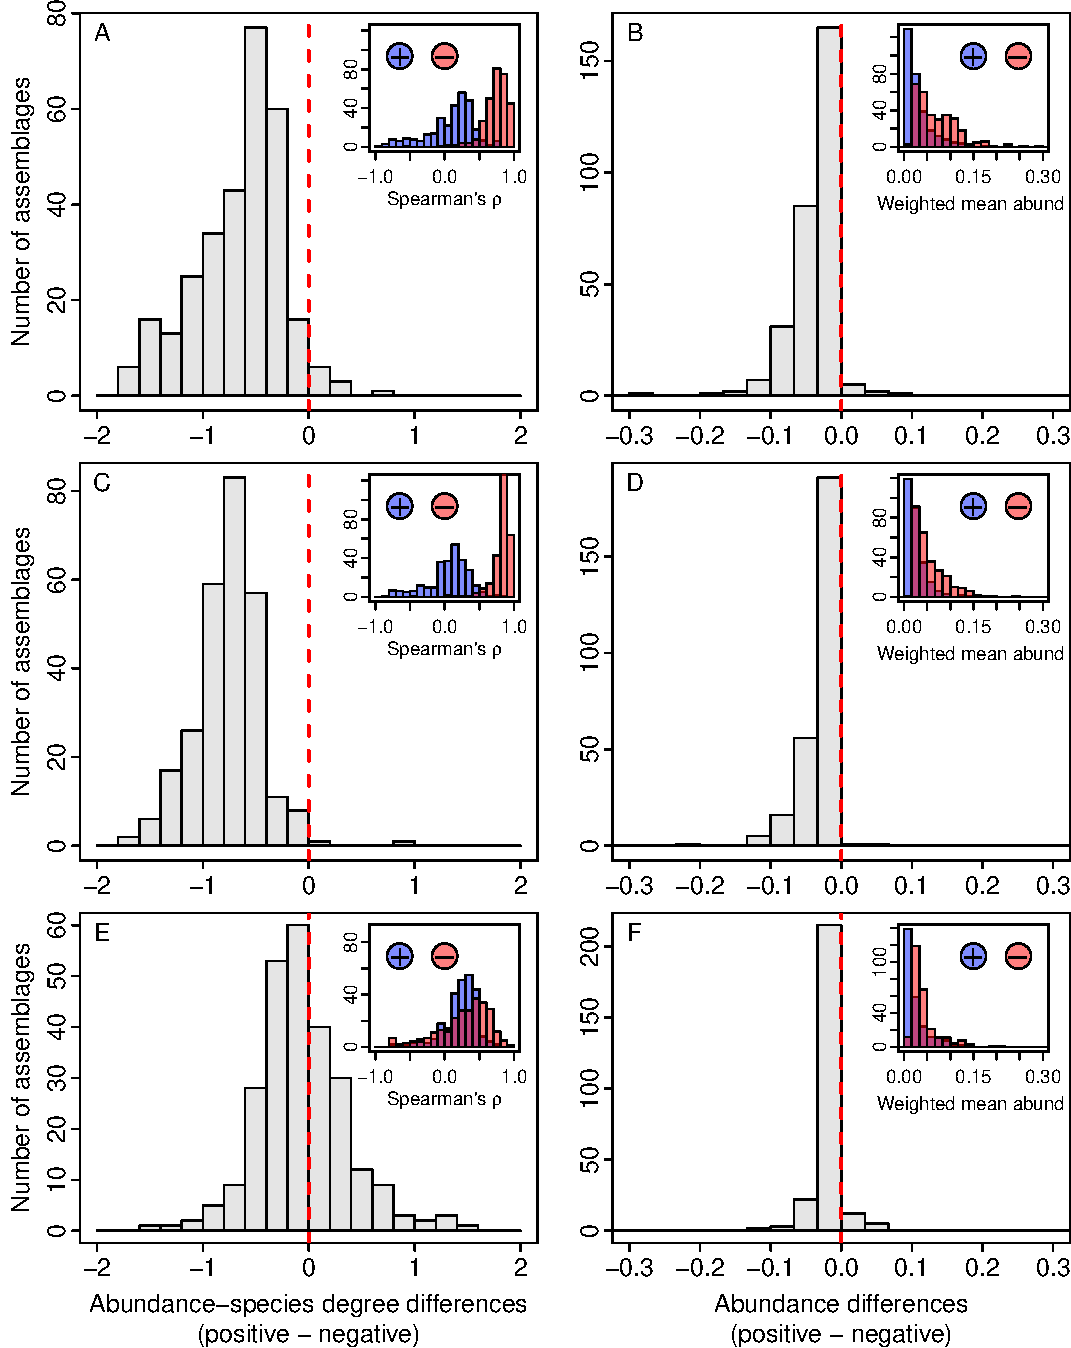
\includegraphics{RarePlusComMinus_files/figure-latex/fig_plusMinus-1} 

}

\caption{Distributions of correlations between network centrality and abundance (left panels) and weighted mean abundance by network type (right panels). The results of CEA Figure 2(B-C) are reproduced in this figure panels A-B; panels C-D show data simulated with a negative binomial SSAD and no species interactions; panels E-F show data simulated with a Poisson SSAD and again no species interactions. \label{fig:plusMinus}}\label{fig:fig_plusMinus}
\end{figure}

Figure \ref{fig:plusMinus} shows that with a negative binomial SSAD, the
simulated data closely match the observed findings. This correspondence
largely dissapears when we instead use a Poisson SSAD, highlighting the
importance of spatial aggregation in driving the artifactual results.
However, we still observe a slight skew toward rare species being
slighly more prevelent with positive interactions (Fig.
\ref{fig:plusMinus}F).

These findings do not depend on simulating SAD and SSAD shapes from the
data: in Supplementary Figure \ref{fig:simpleSim} I show that the
spurious relationship between abundance and interaction type occurs even
when simulating data from just one arbitrary SAD function with the one
arbitrary spatially clustered SSAD for all species. In this simulation,
again, replacing the spatially clustered SSAD with a Poisson SSAD breaks
the spurious association as in Figure \ref{fig:plusMinus}.

We seek to understand why negative binomial SSADs reproduce the results
while Poisson SSADs fail to. The null model algorithm used here and in
CEA\textsuperscript{5} fixes row and column marginals, but within any
given species, the way its total abundance is allocated across sites by
the null model has a potentially large combinitorial space to explore. I
compare known SSADs to their permuted counterpart in Figure
\ref{fig:ssadPerm} and find that the null model transforms negative
binomial SSADs to a more Poisson shape, while leaving Poisson SSADs
probabilistically unchanged. Specifically, when starting with a negative
binomial SSAD, the null model inflates the number of sites individuals
are allocated to (more similarely to a Poisson SSAD) and consiquently
the inferred \(k\) parameter of these permuted SSADs is increase,
indicating less spatial clustering.

\begin{figure}

{\centering 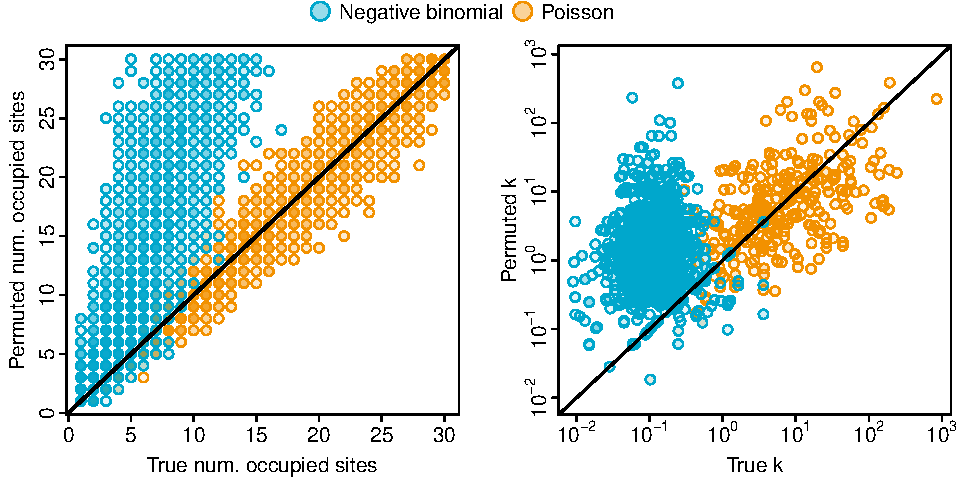
\includegraphics{RarePlusComMinus_files/figure-latex/ssadPerm_plot-1} 

}

\caption{Comparison of true and permuted SSADs in terms of number of sites occupied (A) and inferred clustering parameter $k$ (B). Points are semi-transparent to help display density. Lines are 1:1 lines. \label{fig:ssadPerm}}\label{fig:ssadPerm_plot}
\end{figure}

At a mathematical level, clustered SSADs, compared to spatially even
SSADs, actually increase the probability that rare species will appear
aggregated with each other and common species will appear repelled, this
difference between clustered and even SSADs explains the results.
Consider for example two rare species, one with a single individual and
the other with abundance 5, distributed acorss 5 sites. Their Schoener
similarity is maximized when all individuals occur in the same site,
such as \[
\begin{bmatrix} 1 & 5 \\ 0 & 0 \\ 0 & 0 \\ 0 & 0 \\ 0 & 0 \\ \end{bmatrix}
\] If we define \(Q(x_i; \mu = 1)\) as the probability of observing
\(x_i\) individuals in site \(i\) given an SSAD with mean parameter
\(\mu\), then the probability of the above configuration is
\(Q(5; \mu = 1) Q(0; \mu = 1)^4\). Under a negative binomial SSAD with
\(k = 0.1\) this equals \(4.58 \times 10^{-3}\) whereas under a Poisson
SSAD this equals \(5.61 \times 10^{-5}\).

Converseley, for two common species, say each with abundance 50, an
example configuration that \emph{minimizes} their Schoener similarity
would be \[
\begin{bmatrix} 50 & 0 \\ 0 & 50 \\ 0 & 0 \\ 0 & 0 \\ 0 & 0 \\ \end{bmatrix}
\] We calculate the probability of any such scenerio where no abundances
overlap as \(4 [Q(50; \mu = 10) Q(0; \mu = 10)^{4}]^2\). With a negative
binomial SSAD with \(k = 0.1\) this equals \(1.41 \times 10^{-7}\)
whereas with a Poisson SSAD this equals \(1.61 \times 10^{-72}\).

We can contrast this a configuration that would maximize the Schoener
similarity between these two common species: \[
\begin{bmatrix} 10 & 10 \\ 10 & 10 \\ 10 & 10 \\ 10 & 10 \\ 10 & 10 \\ \end{bmatrix}
\] The probability of this configuration is \(Q(10; \mu = 10)^{10}\)
which, for the same negative binomial equals \(5.76 \times 10^{-22}\),
and for the Poisson equals \(9.40 \times 10^{-10}\).

Thus a clustered SSAD makes rare species appear aggregated, compared to
an even SSAD that, if anything, makes common species appear more
aggregated. Because the null model algorithm preserves even SSADs this
is less of an issue; however, when presented with spatially clustered
abundances, the null model will spuriously identify rare species as
aggregated and common species as repelling each other. This statistical
property accounts for the prevelance of rare species in positive
interaction networks and common species in negative interaction
networks.

Great caution should be used when infering species interactions from
abundance data. At an even more fundamental level than the spurious
association of abundance with interaction type, in the purely random
data sets simulated with a negative binomial SSAD, on average 75\% of
species were placed in positive interaction networks and 74\% in
negative interaction networks with a significance cuttoff of
\(\alpha = 0.05\). With the Poisson SSAD these simulated numbers were
74\% for positive networks and 25\% for negative networks. For the
observed data, on average 73\% of species were placed in positive
interaction networks and 60\% in negative interaction networks. These
are not robust estimates of species interaction.

\clearpage

\section*{References}\label{references}
\addcontentsline{toc}{section}{References}

\hypertarget{refs}{}
\hypertarget{ref-mcgill2005}{}
1. McGill, B. J., Hadly, E. A. \& Maurer, B. A. Community inertia of
quaternary small mammal assemblages in north america. \emph{Proceedings
of the National Academy of Sciences} \textbf{102}, 16701--16706 (2005).

\hypertarget{ref-hutchinson1961}{}
2. Hutchinson, G. E. The paradox of the plankton. \emph{The American
Naturalist} \textbf{95}, 137--145 (1961).

\hypertarget{ref-leigh2004}{}
3. Leigh Jr, E. G. \emph{et al.} Why do some tropical forests have so
many species of trees? \emph{Biotropica} \textbf{36}, 447--473 (2004).

\hypertarget{ref-yenni2012}{}
4. Yenni, G., Adler, P. B. \& Ernest, S. M. Strong self-limitation
promotes the persistence of rare species. \emph{Ecology} \textbf{93},
456--461 (2012).

\hypertarget{ref-calatayud2019}{}
5. Calatayud, J. \emph{et al.} Positive associations among rare species
and their persistence in ecological assemblages. \emph{Nat Ecol Evol}
(2019).

\hypertarget{ref-freilich2018}{}
6. Freilich, M. A., Wieters, E., Broitman, B. R., Marquet, P. A. \&
Navarrete, S. A. Species co-occurrence networks: Can they reveal trophic
and non-trophic interactions in ecological communities? \emph{Ecology}
\textbf{99}, 690--699 (2018).

\hypertarget{ref-carr2019}{}
7. Carr, A., Diener, C., Baliga, N. S. \& Gibbons, S. M. Use and abuse
of correlation analyses in microbial ecology. \emph{The ISME journal}
\textbf{13}, 2647--2655 (2019).

\hypertarget{ref-rajala2019}{}
8. Rajala, T., Olhede, S. C. \& Murrell, D. J. When do we have the power
to detect biological interactions in spatial point patterns?
\emph{Journal of Ecology} \textbf{107}, 711--721 (2019).

\hypertarget{ref-ulrich2010}{}
9. Ulrich, W. \& Gotelli, N. J. Null model analysis of species
associations using abundance data. \emph{Ecology} \textbf{91},
3384--3397 (2010).

\hypertarget{ref-ladau2008}{}
10. Ladau, J. Validation of null model tests using neyman--Pearson
hypothesis testing theory. \emph{Theoretical Ecology} \textbf{1},
241--248 (2008).

\hypertarget{ref-ladau2017}{}
11. Ladau, J. The architecture and design of ecological null models.
\emph{bioRxiv} 195131 (2017).

\hypertarget{ref-hubbell2001}{}
12. Hubbell, S. P. \emph{The unified neutral theory of biodiversity and
biogeography}. (Princeton University Press, 2001).

\hypertarget{ref-mcgill2010}{}
13. McGill, B. J. Towards a unification of unified theories of
biodiversity. \emph{Ecology letters} \textbf{13}, 627--642 (2010).

\hypertarget{ref-harte2011}{}
14. Harte, J. \emph{The maximum entropy theory of ecology}. (Oxford
University Press, 2011).

\hypertarget{ref-mcgill2003}{}
15. McGill, B. \& Collins, C. A unified theory for macroecology based on
spatial patterns of abundance. \emph{Evolutionary Ecology Research}
\textbf{5}, 469--492 (2003).

\hypertarget{ref-engen2008}{}
16. Engen, S., Lande, R. \& Sæther, B.-E. A general model for analyzing
taylor's spatial scaling laws. \emph{Ecology} \textbf{89}, 2612--2622
(2008).

\hypertarget{ref-zillio2010}{}
17. Zillio, T. \& He, F. Modeling spatial aggregation of finite
populations. \emph{Ecology} \textbf{91}, 3698--3706 (2010).

\hypertarget{ref-connolly2017}{}
18. Connolly, S. R., Hughes, T. P. \& Bellwood, D. R. A unified model
explains commonness and rarity on coral reefs. \emph{Ecology letters}
\textbf{20}, 477--486 (2017).

\hypertarget{ref-kendall1949}{}
19. Kendall, D. G. Stochastic processes and population growth.
\emph{Journal of the Royal Statistical Society. Series B
(Methodological)} \textbf{11}, 230--282 (1949).

\hypertarget{ref-rcore}{}
20. R Core Team. \emph{R: A language and environment for statistical
computing}. (R Foundation for Statistical Computing, 2018).


\end{document}
